% A LaTeX (non-official) template for ISAE projects reports
% Copyright (C) 2014 Damien Roque
% Version: 0.2
% Author: Damien Roque <damien.roque_AT_isae.fr>

\documentclass{beamer}
\usepackage[utf8]{inputenc}
\usepackage[ngerman]{babel}
\usepackage{palatino}
\usepackage{graphicx}
\graphicspath{{./images/}}
\usepackage{colortbl}
\usepackage{xcolor}
\usepackage{tikz}
\usetikzlibrary{shapes,arrows}
\usetikzlibrary{mindmap,trees}
\usetikzlibrary{calc}
\usepackage{pgfplots}
\pgfplotsset{compat=newest}
\pgfplotsset{plot coordinates/math parser=false}
\newlength\figureheight
\newlength\figurewidth
\usepackage{ifthen}
\usepackage{subfigure}
\usepackage{amsthm}
\usepackage{amsfonts}
\usepackage{amssymb}
\usepackage{amsmath}
\usepackage{eurosym}
\usepackage{wasysym}

% Printing on 2 slides per page
%\pgfpagesuselayout{2 on 1}[a4paper,border shrink=5mm]

% My macros...
\newcommand*{\SET}[1]  {\ensuremath{\boldsymbol{#1}}}
\newcommand*{\VEC}[1]  {\ensuremath{\boldsymbol{#1}}}
\newcommand*{\MAT}[1]  {\ensuremath{\boldsymbol{#1}}}
\newcommand*{\OP}[1]  {\ensuremath{\text{#1}}}
\newcommand*{\NORM}[1]  {\ensuremath{\left\|#1\right\|}}
\newcommand*{\DPR}[2]  {\ensuremath{\left \langle #1,#2 \right \rangle}}
\newcommand*{\calbf}[1]  {\ensuremath{\boldsymbol{\mathcal{#1}}}}
\newcommand*{\shift}[1]  {\ensuremath{\boldsymbol{#1}}}
\newcommand{\eqdef}{\stackrel{\mathrm{def}}{=}}
\newcommand{\argmax}{\operatornamewithlimits{argmax}}
\newcommand{\argmin}{\operatornamewithlimits{argmin}}
\newcommand{\ud}{\, \text{d}}
\newcommand{\vect}{\text{Vect}}
\newcommand{\sinc}{\text{sinc}}
\newcommand{\esp}{\ensuremath{\mathbb{E}}}
\newcommand{\hilbert}{\ensuremath{\mathcal{H}}}
\newcommand{\fourier}{\ensuremath{\mathcal{F}}}
\newcommand{\sgn}{\text{sgn}}
\newcommand{\intTT}{\int_{-T}^{T}}
\newcommand{\intT}{\int_{-\frac{T}{2}}^{\frac{T}{2}}}
\newcommand{\intinf}{\int_{-\infty}^{+\infty}}
\newcommand{\Sh}{\ensuremath{\boldsymbol{S}}}
\newcommand{\Cpx}{\ensuremath{\mathbb{C}}}
\newcommand{\R}{\ensuremath{\mathbb{R}}}
\newcommand{\Z}{\ensuremath{\mathbb{Z}}}
\newcommand{\N}{\ensuremath{\mathbb{N}}}
\newcommand{\K}{\ensuremath{\mathbb{K}}}
\newcommand{\reel}{\mathcal{R}}
\newcommand{\imag}{\mathcal{I}}
\newcommand{\cmnr}{c_{m,n}^\reel}
\newcommand{\cmni}{c_{m,n}^\imag}
\newcommand{\cnr}{c_{n}^\reel}
\newcommand{\cni}{c_{n}^\imag}
\newcommand{\LR}{\mathcal{L}_2(\R)}
\newcommand{\tproto}{g}
\newcommand{\rproto}{\check{g}}
\newcommand{\Tproto}{G}
\newcommand{\Rproto}{\check{G}}

%\theoremstyle{definition}
%\newtheorem{definition}{Définition}[subsection]

\theoremstyle{remark}
\newtheorem{remarque}{Remarque}[subsection]

\theoremstyle{plain}
\newtheorem{propriete}{Propriété}[subsection]
\newtheorem{exemple}{Exemple}[subsection]

% Choosing a main theme and a color theme
\mode<presentation> {
  %\usetheme{Warsaw}
  \usetheme{Madrid}
  %\usetheme{Frankfurt}
  \usecolortheme{seahorse}
}


\addtobeamertemplate{frametitle}{}{%
\vskip-1em
\begin{tikzpicture}[remember picture,overlay]
\node[anchor=north east,yshift=4pt] at (current page.north east) {
\includegraphics[height=0.8cm]{images/logo-isae-long-sans-texte}};
\end{tikzpicture}}

\title[Recap keys \& console]{Recap Taster und Console}

\author[Tobias Kreienbühl \& Silvan Ritz]{\small Tobias Kreienbühl, Silvan Ritz}

%\date{\today}

% Clear the navigation bar
\setbeamertemplate{navigation symbols}{}
 
%\subject{Sujet de la présentation}

\begin{document}

\begin{frame}
\titlepage
\end{frame}


\begin{frame}
  \frametitle{Plan}
  \small
  \tableofcontents
  \normalsize
\end{frame}

% Recall the outline at each section
\AtBeginSection[]
{%
\begin{frame}
  \frametitle{Ablauf}
  \small
  %\tableofcontents[hideothersubsections]
  \tableofcontents[currentsection,hideothersections]
  %\tableofcontents[currentsubsection]
  \normalsize
\end{frame}
}

\section{Keys}
% !TEX root = isae-beamer-template.tex

% Recall the outline at each section
\begin{frame}
  \frametitle{Definierter Zustand am Eingangspin}
	    \begin{column}{1\linewidth}
	    	Damit immer ein definierter Zustand am Eingang ist:
	    	\begin{center}
	    		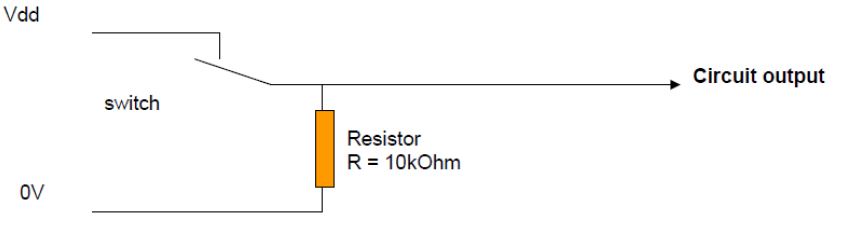
\includegraphics[width=1\textwidth]{images/Pullup.PNG}
	    	\end{center}
	    \end{column}
\end{frame}


\begin{frame}
	\frametitle{Definierter Zustand am Eingangspin}
	\begin{column}{1\linewidth}
		Externer oder interner Pull Widerstand benutzen.\\
		Bei Roboter V2, interne Pull Widerstände aktivieren.
		\begin{center}
			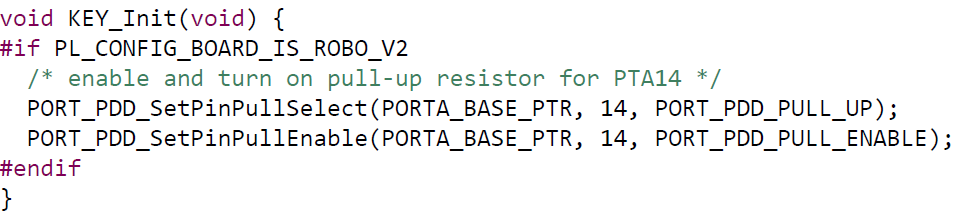
\includegraphics[width=1\textwidth]{images/ROBOV2.PNG}
		\end{center}
	\end{column}
\end{frame}

\begin{frame}
	\frametitle{Zustand einlesen, über Polling}
	\begin{column}{1\linewidth}
		Häufiges Abfragen der Tastereingänge.\\
		\begin{center}
			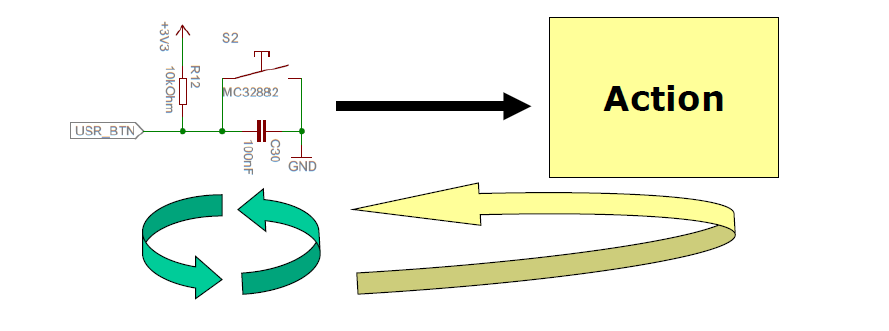
\includegraphics[width=1\textwidth]{images/Polling.PNG}
		\end{center}
	\end{column}
\end{frame}

\begin{frame}
	\frametitle{Zustand einlesen, über Interrupts}
	\begin{column}{1\linewidth}
		Kein Pollig, Interrupt bei Änderung.\\
		Pin muss Interrupt generieren können.
		\begin{center}
			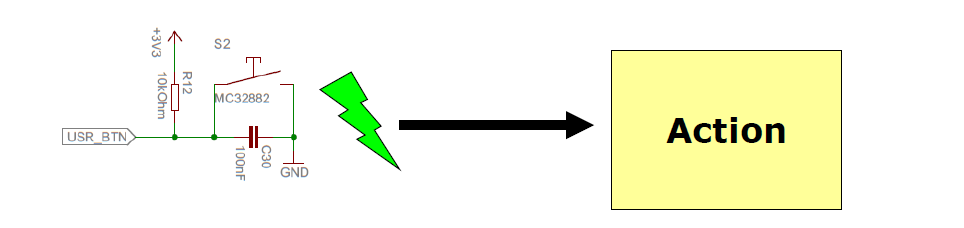
\includegraphics[width=1\textwidth]{images/Interrupt.PNG}
		\end{center}
	\end{column}
\end{frame}

\begin{frame}
	\frametitle{Ablauf mit Polling}
	\begin{column}{1\linewidth}
		\begin{center}
			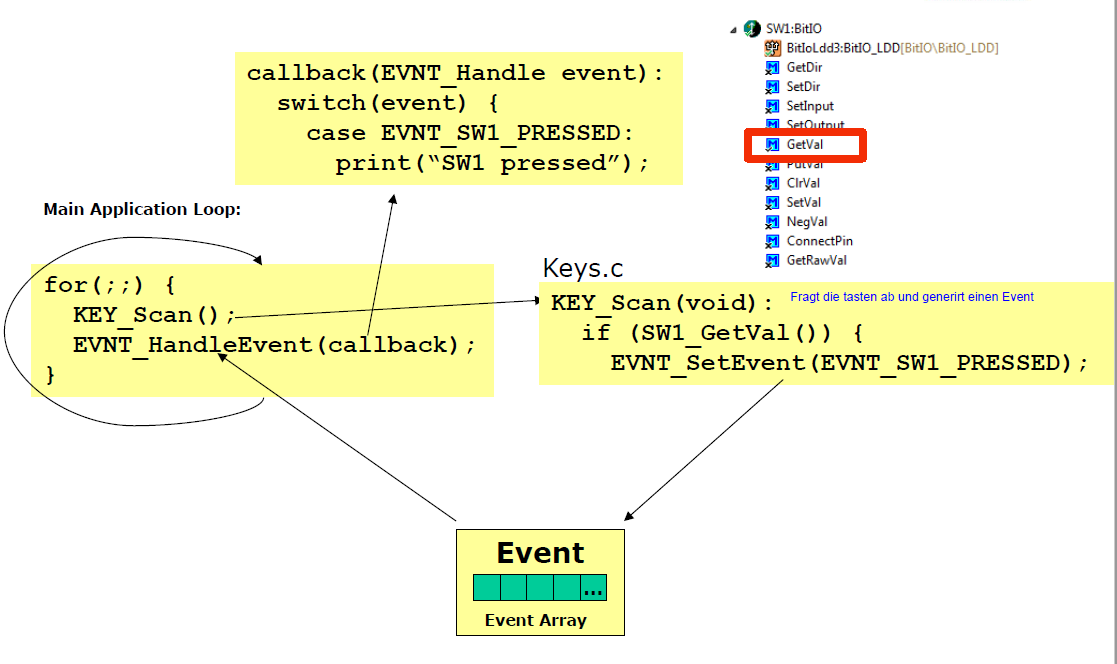
\includegraphics[width=1\textwidth]{images/Taster_Polling.PNG}
		\end{center}
	\end{column}
\end{frame}

\begin{frame}
	\frametitle{Ablauf mit Interrupts}
	\begin{column}{1\linewidth}
		\begin{center}
			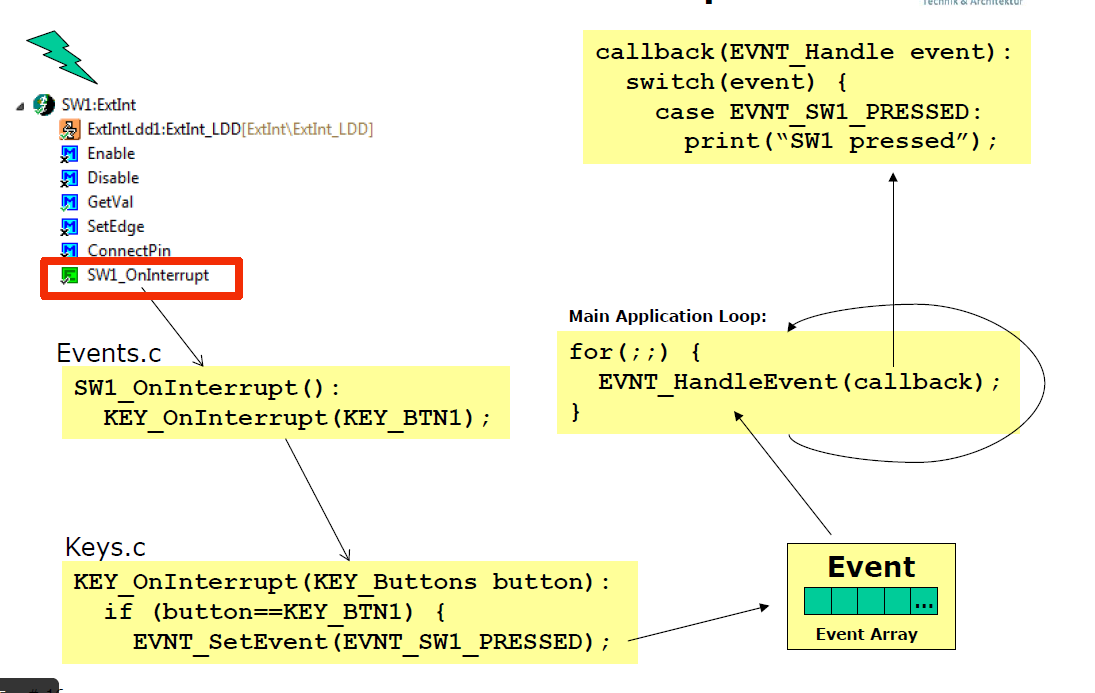
\includegraphics[width=1\textwidth]{images/Intrerrupt_Routine.PNG}
		\end{center}
	\end{column}
\end{frame}
\section{Console}
% !TEX root = isae-beamer-template.tex

% Recall the outline at each section
\begin{frame}
  \frametitle{Serielle Kommunikation über UART}
	    \begin{column}{1\linewidth}
	    	Übersicht über die Hardware-Anbindung UART:\\
	    	Achtung: Robo V1 über \textbf{Segger RTT}
	    	\begin{center}
	    		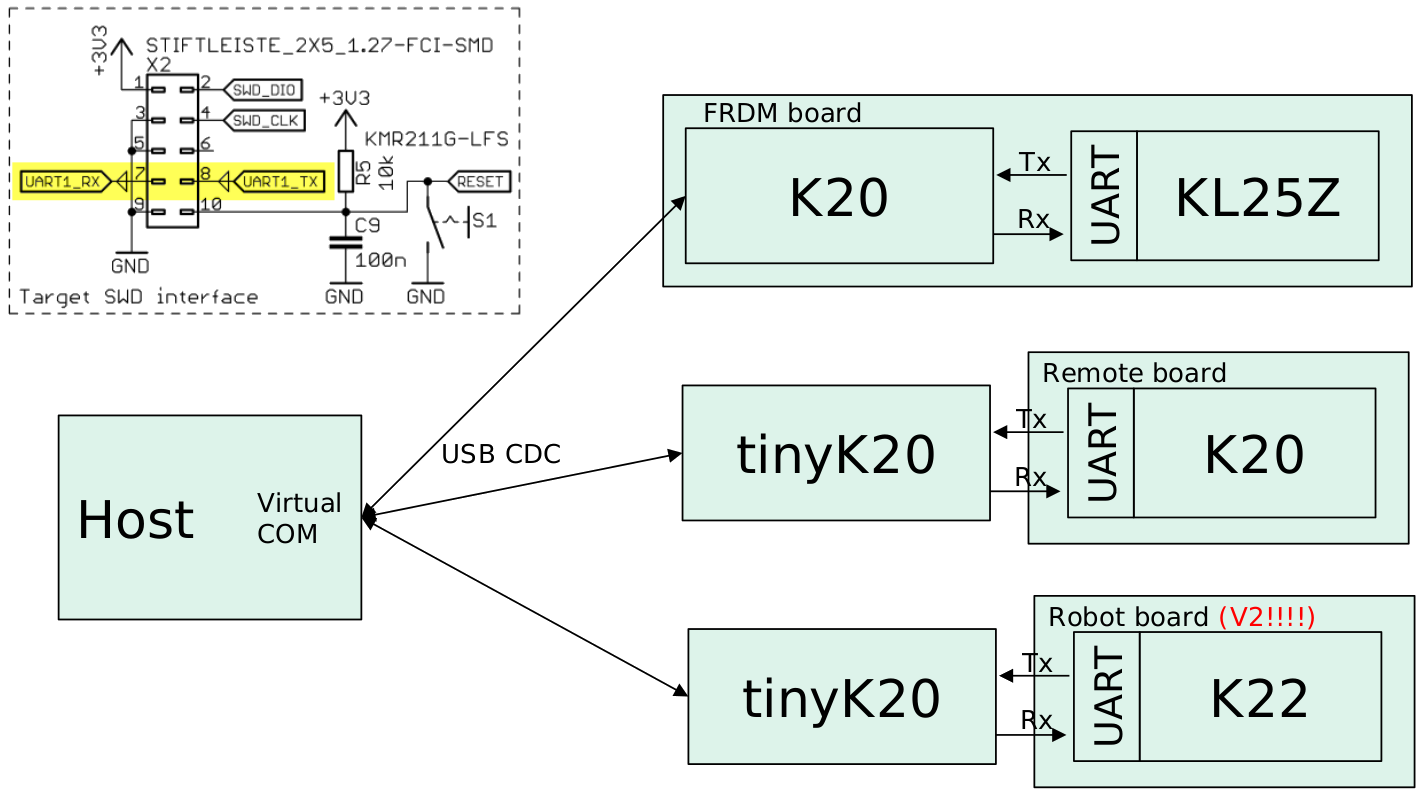
\includegraphics[width=0.8\textwidth]{images/UART_HW_Mapping.png}
	    	\end{center}
	    \end{column}
\end{frame}

\begin{frame}
  \frametitle{Processor Expert Komponenten}
  	\begin{columns}
	    \begin{column}{0.45\linewidth}
	    	\begin{itemize}
	    	\item CLS1:Shell in Processor Expert
	    	\item Blockierendes Senden einschalten
	    	\item WAIT1 verwenden
	    	\item Timeout: Wartezeit zwischen dem Senden. \\0 = blockierend
	    	\item Wait Time: Wenn der Puffer voll ist, wie lange soll gewartet werden?
	    	\item Console Interface: AS1
	    	\end{itemize}
	    \end{column}
	    \begin{column}{0.45\linewidth}
	    	\begin{center}
	    		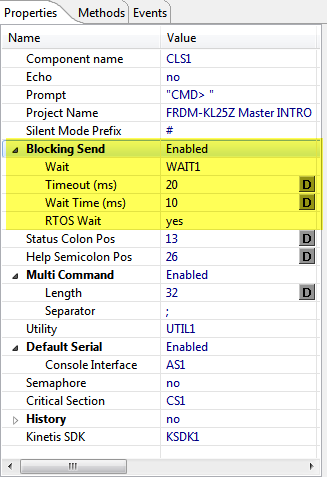
\includegraphics[width=0.8\textwidth]{images/CLS1_shell.png}
	    	\end{center}
	    \end{column}
	\end{columns}
\end{frame}

\begin{frame}
  \frametitle{AS1 Einstellungen}
  	\begin{columns}
	    \begin{column}{0.45\linewidth}
	    	\begin{itemize}
	    	\item Channel: UART0
	    	\item Input buffer size: 32Bit empfohlen
	    	\item Output buffer size: 32Bit empfohlen
	    	\item Receiver: UART0\_RX
	    	\item Transmitter: UART0\_TX
	    	\item Baudrate setzen und mit Terminal abgleichen
	    	\end{itemize}
	    \end{column}
	    \begin{column}{0.45\linewidth}
	    	\begin{center}
	    		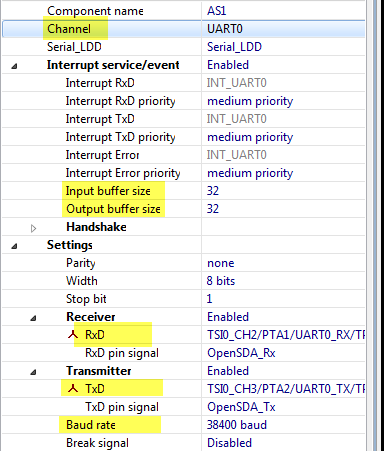
\includegraphics[width=1\textwidth]{images/CLS1_shell_2.png}
	    	\end{center}
	    \end{column}
	\end{columns}
\end{frame}

\begin{frame}[fragile]
  \frametitle{Anschluss am PC/ Notebook}
	    \begin{column}{1\linewidth}
	    	\textbf{Port finden bei Windows:}\\
	    	\begin{center}
	    		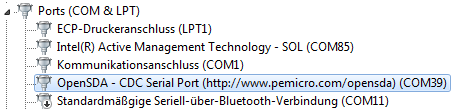
\includegraphics[width=0.7\textwidth]{images/COM_Windows.png}
	    	\end{center}
	    	Achtung: Bei Windows 7 kann es passieren, dass der Port blockiert!\\[0.2cm]
	    	\textbf{Bei Linux:}\\
	    	Terminal öffnen und den untenstehenden Befehl ausführen.
			\begin{verbatim}
				dmesg | grep tty
			\end{verbatim}
			\begin{center}	    	
	    		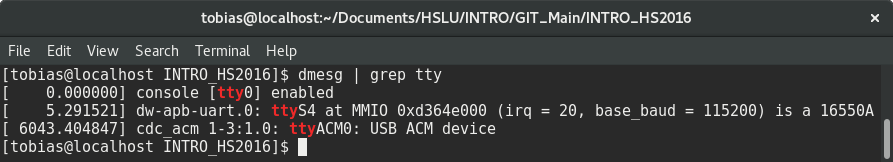
\includegraphics[width=0.7\textwidth]{images/Console_Result_dmesc.png}
	    	\end{center}
	    \end{column}
\end{frame}

\begin{frame}
  \frametitle{Shell Standard I/O}
	    \begin{column}{1\linewidth}
	    	\textbf{I/O Strukturen mit Callback}\\
			\begin{itemize}
			\item \textbf{Stdin}: Zeichen (char) lesen
			\item \textbf{Stdout}: Zeichen schreiben
			\item \textbf{Stderr}: Zeichen schreiben
			\item \textbf{KeyPressed}: Zeichen anstehend in Stdin?
			\end{itemize}
	    	\textbf{Zeichenketten (Strings) und Zahlen senden (nicht printf):}
			\begin{center}	    	
	    		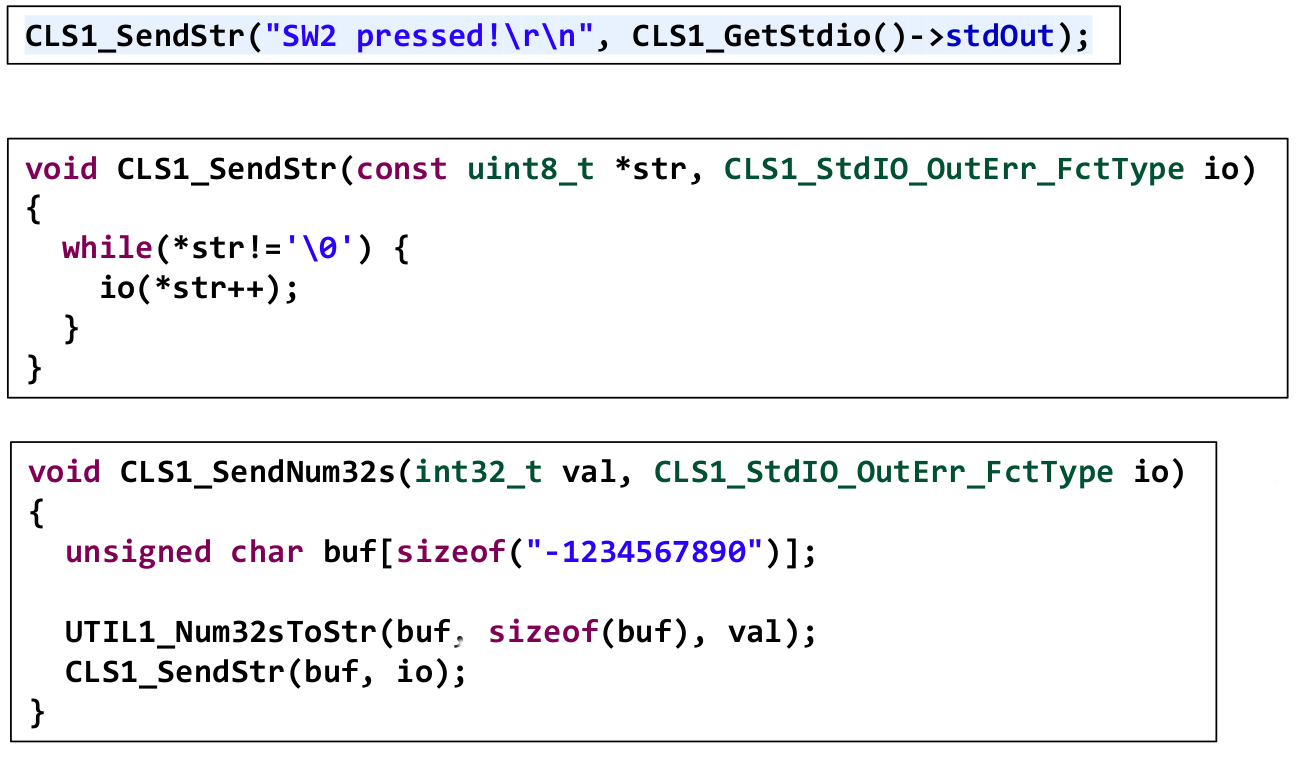
\includegraphics[width=0.6\textwidth]{images/Write_chars.png}
	    	\end{center}	    	
	    \end{column}
\end{frame}
\section{Fragen}
% !TEX root = isae-beamer-template.tex

% Recall the outline at each section
\begin{frame}
  \frametitle{Fragen}
	    \begin{column}{1\linewidth}
		Philipp hat einen Taster auf seinem Robo V2 in Betrieb genommen. Er hat die Interrupt’s eingeschaltet und möchte einen Interrupt wenn der Taster gedrückt ist. Er bekommt aber unregelmässig Interrupt's, ohne das der Taster gedrückt worden ist. An was könnte das liegen?
	    \end{column}
\end{frame}

\begin{frame}
	\frametitle{Fragen}
	\begin{column}{1\linewidth}
		Die Pull- Widerstände sind nicht eingeschaltet. Somit ist der Zustand zwischen den Tastendrücken nicht definiert und so kann es zu ungewollten Interrupts kommen. 
	\end{column}
\end{frame}

\begin{frame}
	\frametitle{Fragen}
	\begin{column}{1\linewidth}
		Jonas liest den Taster mit Polling ein. Am Anfang des Projektes funktioniert alles wunderbar. Aber im laufe des Projektes erkennt das Programm nicht mehr alle Tastendrücke. An was könnte das liegen?
	\end{column}
\end{frame}

\begin{frame}
	\frametitle{Fragen}
	\begin{column}{1\linewidth}
		Wenn über polling Taster eingelesen werden, muss sichergestellt werden, dass die Pollingfunktion genug häufig Aufgerufen wird. Ist dies nicht der Fall, können Tastendrücke verloren gehen. (Am Anfang des Projektes hatte die Pollingfunktion genug Rechenzeit. Aber mit dem wachsen des Projektes hat diese Funktion nun weniger Rechenzeit.)
	\end{column}
\end{frame}

\begin{frame}
	\frametitle{Fragen}
	\begin{column}{1\linewidth}
	Nico wechselt von dem Roboterboard V1 zur V2. Er hat ein Testprogramm geschrieben, welche ihm die Anzahl Tastendrücke zählt. Auf dem Robo V1 hat es gut funktioniert, aber auf dem V2 hat er zu viele Tastendrücke registriert. Was ist bei V2 anders, und wie könnte Nico es trotzdem zum laufen bringen? (Die Pull-Widerstände sind aktiviert)
	\end{column}
\end{frame}

\begin{frame}
	\frametitle{Fragen}
	\begin{column}{1\linewidth}
		Der Robo V1 hat einen Entprellungskondensator am Taster. Der V2 hat dies nicht. Da Nico den Taster nicht Softwaremässig entprellt hat, zählt er zuviele Tastendrücke.
	\end{column}
\end{frame}

\newcounter{lastframe}
\setcounter{lastframe}{\insertframenumber}
\setcounter{framenumber}{\thelastframe}

\end{document}
